\label{Chapter:Automated Guided Jumping for Navigation}
In this chapter we will start by discussing the interaction design for an automated guided jumping navigation technique that would meet the research questions referenced in \ref{section:GJM Conclusion}. This will be followed by details about development of the technique which can be divided into three parts; the setup of an environment and narrative structure for using this technique, development of automated jumping and finally how to make the jumps comprehensible to users. 

\section{Interaction Design}
\label{section AGJN: Interaction Design}
Looking at the use cases and motivation discussed in Chapter \ref{Chapter:Guided Jumping Motivation} we will first lay out a scenario in which our technique would be used and then go through the interaction design of the technique based on this scenario.
\subsection{Scenario}
\label{subsection AGJN ID: Scenario}
We developed our automated guided jumping navigation technique  for a virtual tour of an indoor space which a user can do alone without a tour guide. There is potential to think of how this can be extended to a virtual tour of an indoor space for a group of users without a tour guide as well. The goal of this virtual tour would be to explore specific objects and exhibits that could have a similar theme that a user is interested it and learn about them while also remembering what they have seen and where they saw it. 
\subsection{Exploration Steps}
Figure 
%\vspace{0.5cm}
%
\begin{figure}[]
  \centering
  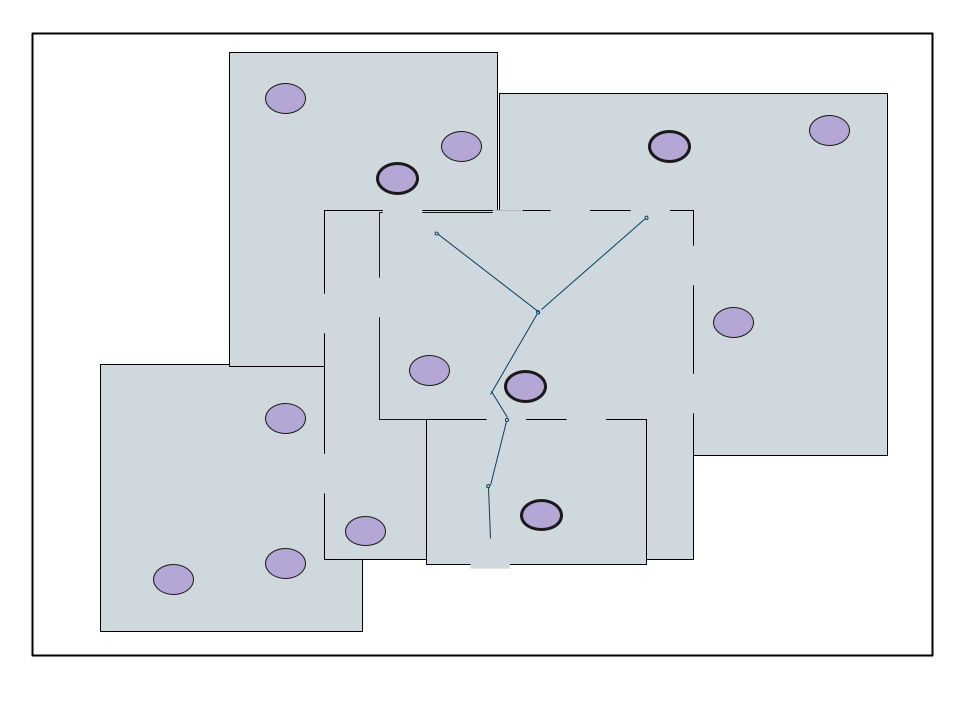
\includegraphics[width=0.5\textwidth]{images/interaction-design-layout.png}
  \caption{This is an example ToDo picture.}
  \label{fig:interaction-design-layout}
\end{figure}

\begin{figure}[]
	\centering
	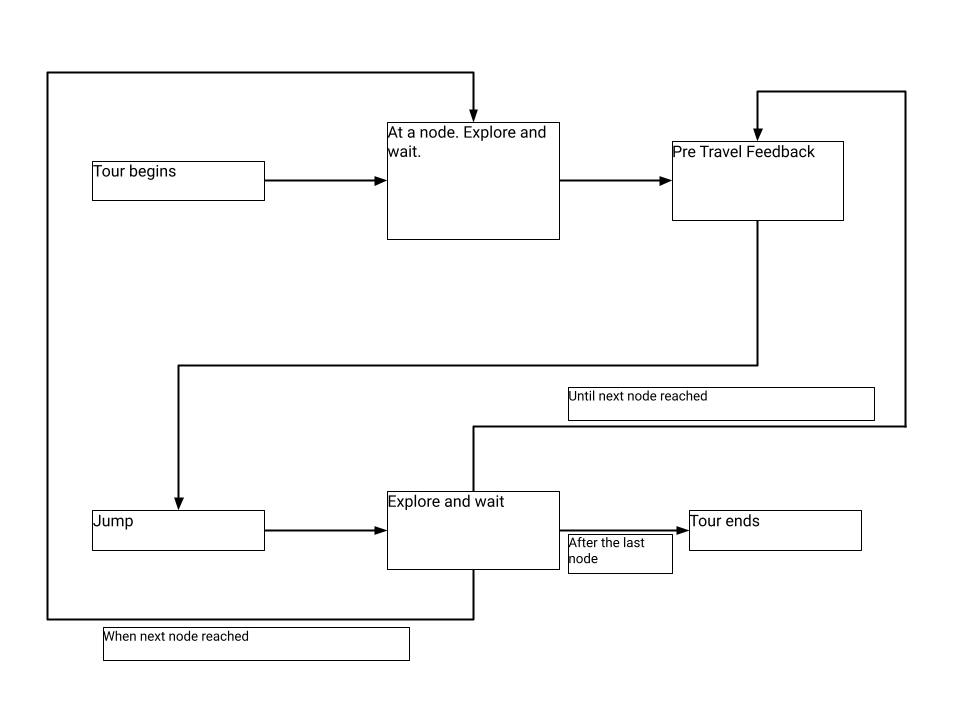
\includegraphics[width=0.5\textwidth]{images/interaction-design-steps.png}
	\caption{This is an example ToDo picture.}
	\label{fig:interaction-design-steps}
\end{figure}
\section{Environment Setup}
\label{section AGJN: Environment Setup}
\section{Automated Jumping}
\label{section AGJN: Automated Jumping}
%\section{Gesture Control}
%\label{section AGJN: Gesture Control}
\section{Comprehensibility of Jumps}
\label{section AGJN: Comprehensibility of Jumps}